\section{Experimental Setup}\label{sec:setup}

\subsection{Examples}
The study uses the regression examples distributed with the \texttt{mggp} package~\cite{mggpy}
(Table~\ref{tab:setup}, Fig.~\ref{fig:data}); the classification mode of the package returns a single objective and is
not considered. Example E1 is the tutorial system
\begin{equation}
y(k)=0.65\,y(k-1)+0.35\,u(k)+0.10\,u(k)\,y(k-1),
\label{eq:tutorial}
\end{equation}
excited by $u=\sin t+0.25\sin 3t$ over $300$ samples, of which the first $70\%$ are used for identification and the
remainder for validation. Example E2 adds white Gaussian measurement noise with standard deviation $0.02$ to the
output of E1. Example E3 uses the package simulator of the Bouc--Wen hysteresis model~\cite{IR2007}, $y=d_p u-h$ with
$\dot h=A\dot u-\beta|\dot u|h-\gamma\dot u|h|$, $A=0.9$, $\beta=\gamma=0.008$ and $d_p=1.6$, integrated by fourth-order
Runge--Kutta with a step of $1$~ms. Identification uses a $1$~Hz sinusoid whose amplitude grows linearly from $20$ to $50$
over $6$~s, and validation a $0.8$~Hz sinusoid of amplitude $45$ over $4$~s; both are decimated by $20$.

\begin{table}[!htbp]
\centering
\caption{Examples and search settings; $C_\mathrm{ref}$ for $\rho=1$ (common: population 100, 50 generations, crossover 0.9, initial mutation 0.2; baseline elite retention 10\%, multiple-shooting horizon $K=20$, primitives \texttt{mul} and $q^{-j}$).}
\label{tab:setup}
\setlength{\tabcolsep}{4pt}
\begin{tabular}{lcccccc}
\toprule
Example & $N_\mathrm{id}$ & $N_\mathrm{val}$ & genes & height & $j_{\max}$ & $C_\mathrm{ref}$ \\
\midrule
E1 Tutorial (noise-free) & 210 & 90 & 5 & 2 & 2 & 25 \\
E2 Tutorial (noisy) & 210 & 90 & 5 & 2 & 2 & 25 \\
E3 Bouc--Wen hysteresis & 300 & 200 & 8 & 3 & 3 & 72 \\
\bottomrule
\end{tabular}
\end{table}


\begin{figure*}[!htbp]
\centering
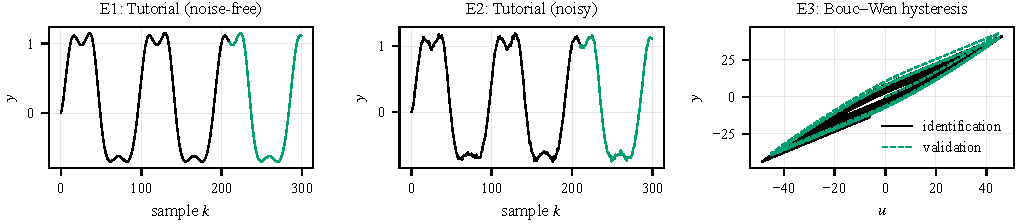
\includegraphics[width=\textwidth]{figures/fig_data.pdf}
\caption{Identification and validation data of the three examples. E3 is shown in the input--output plane, where the
loops reveal the hysteresis.}
\label{fig:data}
\end{figure*}

\subsection{Common evaluator, selection schemes and search budgets}
SO minimises identification error and delivers its Hall-of-Fame model. MO-lex uses the arithmetic cost as a second fitness component but compares it lexicographically; Green uses Pareto ranking and crowding. All methods use the external corrected evaluator described in Section~\ref{sec:method}, the same examples, least-squares estimator, representation, variation operators and initial rates. Both declared weights are fixed before searching: $\rho=1$ is primary and $\rho_K=729/64$ is the bit-level comparison. SO does not use either cost for selection.

The main comparison uses 100 initial evaluations followed by 49 steps of 90 evaluated offspring, giving exactly 4,510 fitness calls per run, including unchanged offspring and failures. The 50 recorded generations include the initial population. The initial mutation probability is 0.2; at nine-generation checkpoints it increases by 0.1, up to 0.9, when improvement is below 5\%. Baseline survival retains 10\% elites, whereas Pareto configurations use union-based survival.

Two additional Pareto configurations minimise distinct canonical terms or all representation nodes, respectively, alongside identification error. Node counting includes duplicate genes; structural de-duplication retains the smallest representation for this ablation. The same arithmetic cost and identification-only $\tau$-rule assess the delivered sets of every configuration. Each of the five configurations uses 30 independent seeds on each example under both weights (900 runs). A separate native-budget diagnostic retains the original offspring counts and fitness reuse for SO, MO-lex and Green (540 runs); it is not the principal equal-evaluation comparison. The complete study therefore contains 1,440 runs.

\subsection{Assessment and statistical comparisons}
Hypervolume~\cite{ZT1999} is computed in $(C_\rho/C_{\mathrm{ref}},\mathrm{NRMSE})$ with reference $(1,1)$ and the cost bound declared from $G$ genes of degree $2^{h_{\max}}$. Identification and free-run validation hypervolumes assess the same delivered models. Points outside the reference contribute nothing; reference-point sensitivity is analysed separately~\cite{Ishibuchi2018}. The fixed $\tau=0.05$, $\eta=10^{-6}$ rule uses identification data only. Validation initialises the actual maximum delay from measured outputs; non-finite simulations remain failures and are excluded from finite-error medians, with their counts retained.

Comparisons use two-sided Mann--Whitney tests~\cite{MW1947}, Holm correction~\cite{Hol1979} and Vargha--Delaney $A_{12}$~\cite{VD2000}. Seeds index independent runs; method comparisons are not paired. Holm families contain 60 tests per weight in the equal-evaluation arm and 30 in the native diagnostic, covering the tested metrics, examples and comparator configurations. Runtime recorded during concurrent searches is diagnostic; the isolated timing and energy session is reported separately in Section~\ref{sec:energy}.
